\begin{figure}[t]
\centering
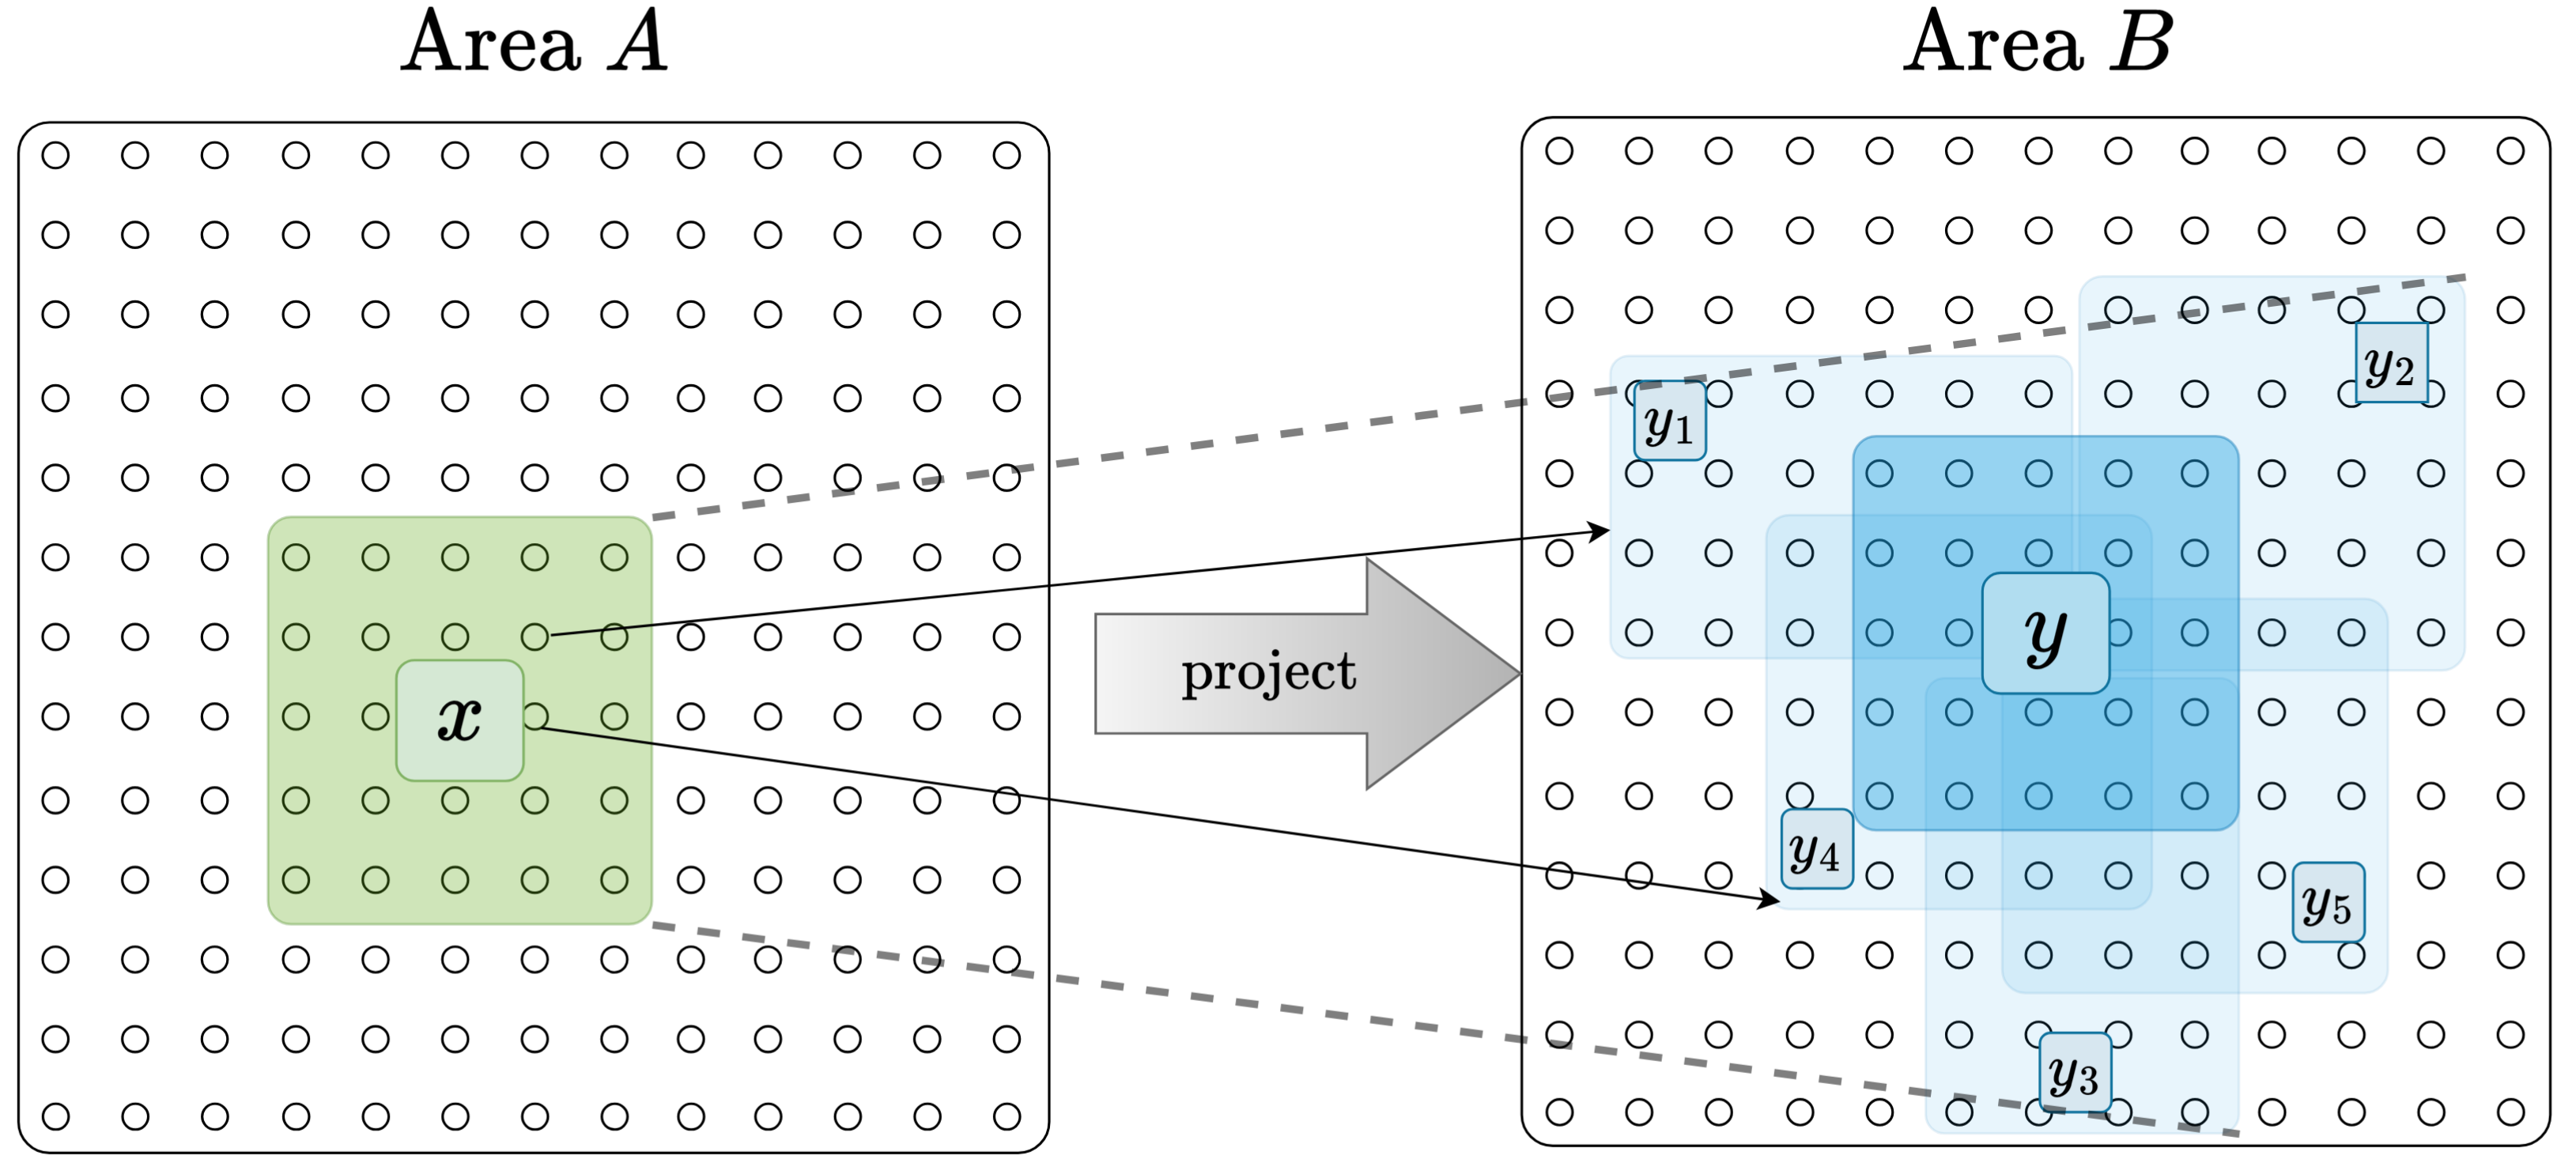
\includegraphics[width=0.9\linewidth]{figures/AC_fundamentals.png}
\caption{Fundamental \textbf{Project} operation of Assembly Calculus. Binary input vectors are projected into a neural area where the $k$-cap operation selects the top-$k$ most activated neurons to form a sparse assembly. Recurrent plasticity strengthens connections between co-active neurons, causing assemblies to stabilise over repeated presentations of the same input.}
\vspace{-10pt}
\label{fig:ac_fundamentals}
\end{figure}
